\documentclass[10pt]{beamer}
\usepackage{amsmath}
\usefonttheme{professionalfonts} % using non standard fonts for beamer
\usefonttheme{serif} % default family is serif\
\usepackage{mathtools}
%\documentclass[12pt]{beamerthemeSam.sty}
\usepackage{epsf}
%\usepackage{pstricks}
%\usepackage[orientation=portrait,size=A4]{beamerposter}
\geometry{paperwidth=160mm,paperheight=120mm}
%DT favorite definitions
\def\LL{\left\langle}	% left angle bracket
\def\RR{\right\rangle}	% right angle bracket
\def\LP{\left(}		% left parenthesis
\def\RP{\right)}	% right parenthesis
\def\LB{\left\{}	% left curly bracket
\def\RB{\right\}}	% right curly bracket
\def\PAR#1#2{ {{\partial #1}\over{\partial #2}} }
\def\PARTWO#1#2{ {{\partial^2 #1}\over{\partial #2}^2} }
\def\PARTWOMIX#1#2#3{ {{\partial^2 #1}\over{\partial #2 \partial #3}} }

\def\rightpartial{{\overrightarrow\partial}}
\def\leftpartial{{\overleftarrow\partial}}
\def\diffpartial{\buildrel\leftrightarrow\over\partial}

\def\BI{\begin{itemize}}
	\def\EI{\end{itemize}}
\def\BE{\begin{displaymath}}
	\def\EE{\end{displaymath}}
\def\BEA{\begin{eqnarray*}}
	\def\EEA{\end{eqnarray*}}
\def\BNEA{\begin{eqnarray}}
	\def\ENEA{\end{eqnarray}}
\def\EL{\nonumber\\}
\def\BS{\bigskip}


\newcommand{\map}[1]{\frame{\frametitle{\textbf{Course map}}
		\centerline{\includegraphics[height=0.86\paperheight]{../../map/#1.png}}}}
\newcommand{\wmap}[1]{\frame{\frametitle{\textbf{Course map}}
		\centerline{\includegraphics[width=0.96\paperwidth]{../../map/#1.png}}}}

\newcommand{\etal}{{\it et al.}}
\newcommand{\gbeta}{6/g^2}
\newcommand{\la}[1]{\label{#1}}
\newcommand{\ie}{{\em i.e.\ }}
\newcommand{\eg}{{\em e.\,g.\ }}
\newcommand{\cf}{cf.\ }
\newcommand{\etc}{etc.\ }
\newcommand{\atantwo}{{\rm atan2}}
\newcommand{\Tr}{{\rm Tr}}
\def\BS{\bigskip}
\def\BC{\begin{center}}
	\def\EC{\end{center}}
\def\BCC{\begin{columns}}
	\def\ECC{\end{columns}}
\def\HC{\column{0.5\textwidth}}
\newcommand{\dt}{\Delta t}
\newcommand{\op}{{\cal O}}
\newcommand{\msbar}{{\overline{\rm MS}}}
\def\chpt{\raise0.4ex\hbox{$\chi$}PT}
\def\schpt{S\raise0.4ex\hbox{$\chi$}PT}
\def\MeV{{\rm Me\!V}}
\def\GeV{{\rm Ge\!V}}

%AB: my color definitions
%\definecolor{mygarnet}{rgb}{0.445,0.184,0.215}
%\definecolor{mygold}{rgb}{0.848,0.848,0.098}
%\definecolor{myg2g}{rgb}{0.647,0.316,0.157}
\definecolor{abtitlecolor}{rgb}{0.0,0.255,0.494}
\definecolor{absecondarycolor}{rgb}{0.0,0.416,0.804}
\definecolor{abprimarycolor}{rgb}{1.0,0.686,0.0}
\definecolor{Red}           {cmyk}{0,1,1,0}
\definecolor{Grey}           {cmyk}{.7,.7,.7,0}
\definecolor{Lg}           {cmyk}{.4,.4,.4,0}
\definecolor{Blue}          {cmyk}{1,1,0,0}
\definecolor{Green}         {cmyk}{1,0,1,0}
\definecolor{Brown}         {cmyk}{0,0.81,1,0.60}
\definecolor{Black}         {cmyk}{0,0,0,1}
\definecolor{A}{rgb}{0.8,0.0,0.0}
\definecolor{B}{rgb}{0.0,0.6,0.0}
\definecolor{C}{rgb}{0.6,0.6,0.0}
\definecolor{D}{rgb}{0.0,0.0,0.5}
\definecolor{E}{rgb}{0.4,0.4,0.4}


\usetheme{Madrid}


%AB: redefinition of beamer colors
%\setbeamercolor{palette tertiary}{fg=white,bg=mygarnet}
%\setbeamercolor{palette secondary}{fg=white,bg=myg2g}
%\setbeamercolor{palette primary}{fg=black,bg=mygold}
\setbeamercolor{title}{fg=abtitlecolor}
\setbeamercolor{frametitle}{fg=abtitlecolor}
\setbeamercolor{palette tertiary}{fg=white,bg=abtitlecolor}
\setbeamercolor{palette secondary}{fg=white,bg=absecondarycolor}
\setbeamercolor{palette primary}{fg=black,bg=abprimarycolor}
\setbeamercolor{structure}{fg=abtitlecolor}

\setbeamerfont{section in toc}{series=\bfseries}

%AB: remove navigation icons
\beamertemplatenavigationsymbolsempty
\title{
	\textbf {Rotational motion}\\
	%\centerline{}
	%\centering
	%\vspace{-0.0in}
	%\includegraphics[width=0.3\textwidth]{propvalues_0093.pdf}
	%\vspace{-0.3in}\\
	%\label{intrograph}
}

\author[W. Freeman] {Physics 211\\Syracuse University, Physics 211 Spring 2023\\Walter Freeman}

\date{\today}

\begin{document}
	
	\frame{\titlepage}
	
	\frame{\frametitle{\textbf{Announcements}}
		\BI
		\item{No recitation today or tomorrow}
		\item{Office hours today 3-5pm}
		\item Turn your homework in to your TA's mailbox (in front of room 201 upstairs)
		\EI
	}
	
	\frame{\frametitle{\textbf{An overview of rotational motion}}
		\large
		Everything you've learned about linear motion has a rotational equivalent:
		\BI
		\item{Position, velocity, acceleration $\leftrightarrow$ angle, angular velocity, angular acceleration}
		\item{Kinematics for coordinates  $\leftrightarrow$ kinematics for angles}
		\item{Newton's second law $\leftrightarrow$ Newton's law for rotation}
		\item{Force  $\leftrightarrow$ torque}
		\item{Mass  $\leftrightarrow$ moment of inertia}
		\item{... and others}
		\EI
		
		\bigskip
		
		We're going to go over these things piece by piece -- learning their details as we go.
		
		\bigskip
		
		First, though, you should see the whole picture (and keep it for reference):
		
	}
	
	\frame{
		\begin{center}
			\begin{tabular}{l | l}
				
				\multicolumn{1}{c|}{\Large Translation} & \multicolumn{1}{c}{\Large Rotation} \\
				\\
				\hline
				\hline
				& \\
				Position $\vec s$ & Angle $\theta$ \\
				Velocity $\vec v$ & Angular velocity $\omega$ \\
				Acceleration $\vec a$ & Angular acceleration $\alpha$ \\
				& \\
				\hline
				\hline
				& \\
				Kinematics: $\vec s(t)\frac{1}{2}\vec at^2 + \vec v_0 t + \vec s_0$ & $\theta(t) = \frac{1}{2}\alpha t^2 + \omega_0 t + \theta_0$ \\
				& \\
				\hline
				\hline
				
				& \\
				Force $\vec F$ & Torque $\tau$ \\
				Mass $m$ & Rotational inertia $I$ \\
				Newton's second law $\vec F = m \vec a$ & Newton's second law for rotation $\tau = I \alpha$ \\
				& \\
				
				\hline
				\hline
				
			
				
				& \\
				Momentum $\vec p = m \vec v$ & Angular momentum $L = I\omega$\\
				& \\
				\hline
				\hline
				
				&\\

			Kinetic energy $KE=\frac{1}{2}mv^2$ & Kinetic energy $KE=\frac{1}{2}I\omega^2$ \\
				Work $W = \vec F \cdot \Delta \vec s$ & Work $W = \tau \Delta \theta$ \\
				Power $P = \vec F \cdot \vec v$ & Power $P = \tau \omega$ \\
				& \\
				
				\hline
				\hline
				
		
			\end{tabular}
		\end{center}
	}

\frame{\frametitle{\textbf{Rotational motion and kinematics}}
	\large
	First, we need to describe how rotating objects move.
	
	\BS
	
	Rotational motion can be described separate from its translational motion. 
	
	\BS 
	
	Describing rotation by itself is simple: it's the same as one-dimensional 
	motion (no vectors!)
	
	
	\BS
	
	An example: consider a centrifuge rotating at $\omega=1000 {\rm rad}/{\rm s}$.
	Once its motor is turned off, slows down at $\alpha=-100 {\rm rad/\rm s^2}$.
	How long will it take to stop?
}

\frame{\frametitle{\textbf{Rotational motion and kinematics}}

\begin{minipage}{0.45\textwidth}
		\color{Red}
	A centrifuge rotates at $\omega=1000 \,{\rm rad}/{\rm s}$.
	Once its motor is turned off, slows down at $\alpha=-100 \,{\rm rad/\rm s^2}$.
	How much time will it take to stop, and how many times will it rotate before it does?
	\end{minipage}\hspace{0.09\textwidth}
\pause
\begin{minipage}{0.45\textwidth}
		\color{Green}
	An object moves at $v_0=1000\, {\rm cm}/{\rm s}$.
	It begins to slow down at $a=-100\, {\rm cm/\rm s^2}$.
	How much time will it take to stop, and how far will it move before it does?
\end{minipage}

\begin{minipage}{0.45\textwidth}
	\color{Red}
$$\omega(t) = \omega_0 + \alpha t$$

$$\theta(t) = \theta_0 + \omega_0 t + \frac{1}{2}\alpha t^2$$

\BI
\item $\theta$ is angular position
\item $\omega$ is angular velocity
\item $\alpha$ is angular acceleration
\EI

\end{minipage}\hspace{0.09\textwidth}
\pause
\begin{minipage}{0.45\textwidth}
	\color{Green}
$$v(t) = v_0 + a t$$

$$x(t) = x_0 + v_0 t + \frac{1}{2}a t^2$$

\BI
\item $x$ is position
\item $v$ is velocity
\item $a$ is acceleration
\EI
	
\end{minipage}
}

\frame{\frametitle{\textbf{Most things in rotational motion are very familiar!}}
	Most aspects of rotational dynamics work just like their translational counterparts.
	
	\bigskip\bigskip
	
	The parallels in the previous example hold for most areas of dynamics we will learn about.
	
\bigskip
\bigskip

What about momentum?
}

\frame{\frametitle{\textbf{Angular momentum}}
\large

\begin{align*}
\color{Red}\text{(Momentum)} &= \color{Green}\text{(mass)} &\times& \color{Blue}\text{(velocity)} \\
\color{Red}\text{(Momentum)} &= \color{Green}\text{(how hard an object is to move)} &\times& \color{Blue}\text{(how fast it is moving)} 
\end{align*}

\bigskip\bigskip

\begin{center}
\bf	Can we do something similar for angular momentum?
\end{center}

\begin{align*}
	\color{Red}\text{(Angular momentum)} &= \color{Green}\text{(how hard an object is to turn)} &\times& \color{Blue}\text{(how fast it is turning)} \\
	\color{Red}\text{(Angular momentum)} &= \color{Green}\text{(``moment of inertia'')} &\times& \color{Blue}\text{(angular velocity)} \\
\end{align*}


}

\frame{\frametitle{\textbf{Moment of inertia}}
	
	\centerline{\Large The analogue of mass is called ``moment of inertia'' (letter $I$)}.
	
	\bigskip
	
	\large
	
	\BI
	\item Mass: how hard you have to push on a thing to get it to move
	\item Moment of inertia: how hard you have to twist a thing to get it to turn
	\EI
	
	\bigskip\bigskip
	
	
	\BI
	\large
	\item{More massive things are harder to turn, but that's only part of it}
	\item{The mass {\it distribution} matters, too}
	\item{The further the mass is from the center, the harder it will be to turn}
	\item{The moment of inertia depends on the {\it average squared distance from the center}}
	\EI
	
	\bigskip\pause
	
	\centerline{\Large $I=MR^2$}
	
	\bigskip
	\bigskip
	\bigskip
	
	\centerline{\large (if all the mass is the same distance from the center)}
	\centerline{\large (our demo rods; hoops; rings; bike wheels)}
}


\frame{\frametitle{\textbf{Moment of inertia, other things}}
	\centerline{\Large What about the moment of inertia of other objects?}
	\centerline{\large Requires calculus in general; here are some common ones}
	\centerline{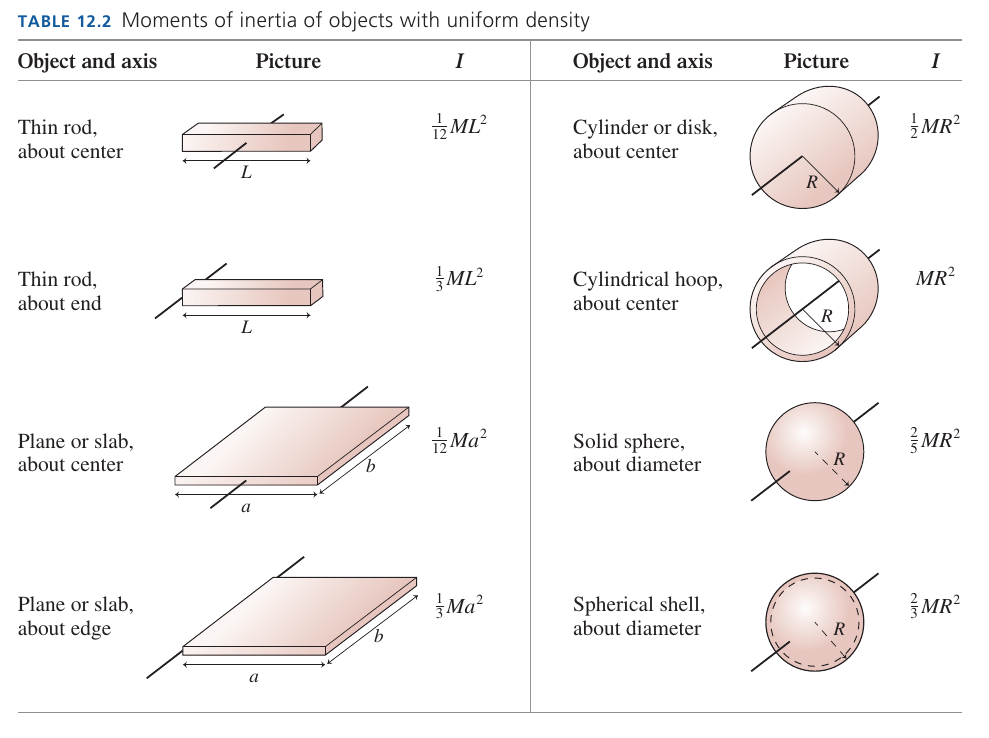
\includegraphics[width=0.7\textwidth]{moment-table.png}}
	
	\BS
	\pause
	\centerline{In general: $I=\lambda MR^2$}
	\centerline{We will always give you $\lambda$ if it's not 1 (i.e. not a ring etc.)}
}


\frame{\frametitle{\textbf{Angular momentum}}
	\begin{columns}
		\column{0.5\textwidth}
		\color{Grey}
		\Large
		\centerline{Translational motion}
		\normalsize
		\BI
		{\color{Red}
			\item{Moving objects have momentum}
			\item{$\vec p = m \vec v$}
			\item{Momentum conserved if there are no external forces}}
		\EI
		\column{0.5\textwidth}
		\color{Grey}
		\Large
		\centerline{Rotational motion}
		\normalsize
		\BI
		{\color{Blue}
			\item{Spinning objects have angular momentum $L$}
			\item{$L = I \omega$}
			\item{Angular momentum conserved if no external twisting forces}}
		\EI
	\end{columns}
	
	\bigskip
	\bigskip
	
	\Large
	\color{Red}
	
	$\rightarrow$ $L = I \omega = $ constant; analogue to conservation of momentum
	
}

\frame{\frametitle{\textbf{Conservation of angular momentum}}
	\large
	We saw that the conservation of momentum was valuable mostly in two sorts of situations:
	
	\BI
	\item{Collisions: two objects strike each other}
	\item{Explosions: one object separates into two}
	\EI
	
	There is a third common case for conservation of angular momentum:
	
	\BI
	\item{Collisions: a child runs and jumps on a merry-go-round}
	\item{Explosions: throwing a ball off-center}
	\item{{\color{Red}A spinning object changes its moment of inertia}}
	\EI
	
	\pause
	\bigskip
	
	This last happens because moment of inertia depends on {\it how the mass is distributed}, not just how much there is!
}

\frame{\frametitle{\textbf{Conservation of angular momentum}}
	
	\Large
	\BC
	
	These problems are approached in exactly the same way as conservation of 
	{\it linear} momentum problems: write down expressions for $L_i$ and $L_f$ 
	and set them equal.
	
	\Huge
	
	$$L = I \omega$$
	
	$$\sum L_i=\sum L_f$$ \\
	
	\EC
}


\frame{
	
	\Large
	
	What will happen when I pull the string, collapsing the ball?
	
	\BI
	\item A: The ball will rotate faster
	\item B: The ball will rotate slower
	\item C: Nothing will happen \pause
	\item The bolt connecting the ball to the ceiling will fail, and the whole thing will fall on my head
	\EI
}



\frame{\frametitle{\textbf{Conservation of angular momentum}}
	\Large
	If I kept the mass of the Earth the same, but enlarged it so that it had twice
	the diameter, how long would a day be?
	
	\BS
	
	(Remember, the total angular momentum, $L=I\omega$, stays the same. The moment of inertia of a ball is $I = \frac{2}{5}mR^2$.)
	
	\BS
	\BS
	
	\Huge
	
	\color{A}A: 6 hours\\
	\color{B}B: 12 hours\\
	\color{C}C: 24 hours\\
	\color{D}D: 48 hours\\
	\color{E}E: 96 hours\\
}



\frame{
	
	\Large
	
	What will happen the person on the platform turns the wheel over?
	
	\BI
	\item A: Nothing will happen
	\item B: They will rotate counterclockwise
	\item C: They will rotate clockwise
	\item D: They will stop rotating
	\EI
}



\frame{\frametitle{\textbf{Angular momentum of a single object}}
	
	\large
	
	A single object moving in a straight line also has angular momentum.
	\Huge
	$$L = mv_\perp r = mvr_\perp$$
	\large
	
	\BS
	\BS
	\BS
	
	\BCC
	\HC
	If we are to trust this relation, then the angular momentum of an object moving 
	with constant $\vec v$ should be constant!
	
	\BS
	
	Is the angular momentum the same at points A and B?
	\HC
	\BC
	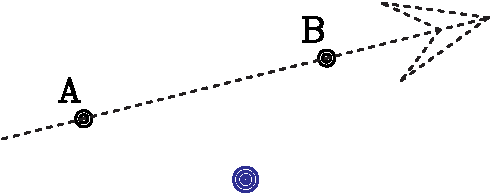
\includegraphics[width=0.8\textwidth]{angmombare-crop.pdf}
	\EC
	\ECC
}


\frame{\frametitle{\textbf{Angular momentum of a single object}}
	
	\large
	
	A single object moving in a straight line also has angular momentum.
	\Huge
	$$L = \color{Lg}mv_\perp r =\color{Red} mvr_\perp$$
	\large
	
	\BS
	\BS
	\BS
	
	\BCC
	\HC
	Is the angular momentum the same at points A and B?
	
	\BS
	
	\color{Red}
	Yes: $r_\perp$ (and $v$) are the same at both points.
	
	\HC
	\BC
	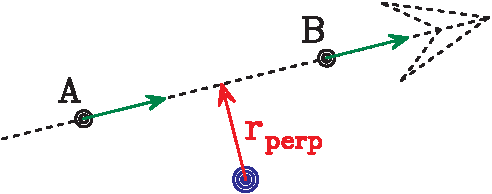
\includegraphics[width=0.8\textwidth]{angmom-crop.pdf}
	\EC
	\ECC
}



\frame{\frametitle{\textbf{Angular momentum demonstrations}}
	
	\Large
	
	What happens to the person on the platform if they catch the ball?
	
	\pause
	
	What happens when they throw it?
}

\frame{\frametitle{\textbf{An example problem}}
	\Large
	A child of mass $m$ runs at speed $v$ straight east and jumps onto a merry-go-round of mass $M$ and radius $R$,
	landing $2/3$ of the way toward the outside. If she lands on the south edge,
	how fast will it be turning once she lands?
	
	\BS
	
	We'll do this together on the document camera.
	
	\pause
	
	\BS\BS
	\BC\it\normalsize
	
	(The solution is on the next slide, for those studying these notes later)
	\EC
}

\frame{\frametitle{\textbf{The solution to our example}}
	\large
	
	We use conservation of angular momentum:
	
	\begin{align*}
		\sum L_i &= \sum L_f \\
		L_{\rm child,\it i}  &= L_{\rm child+disk,\it f}
	\end{align*}
	
	Model the child as a point object moving at a constant velocity:
	$$L_{\rm child,\it i} = mv_\perp r = \frac{2}{3} mvR$$
	
	This gives us $\frac{2}{3}mvR = I_{\rm total} \omega_f$. We now need $I_{\rm total}$.
	
	\medskip
	
	After the child jumps on, $I_{\rm total} = I_{\rm disk} + I_{\rm child} = \frac{1}{2}MR^2 + \frac{2}{3}mR^2$. Thus,
	
	$$\frac{2}{3}mvR = \left(\frac{1}{2}MR^2 + \frac{2}{3}mR^2\right) \omega_f$$
	
	Solve for $\omega_f$:
	
	$$
	\omega_f = \frac{\frac{2}{3}mvR}{\left(\frac{1}{2}MR^2 + \frac{2}{3}mR^2\right)}
	$$
	
	}





\end{document}
